\documentclass{article}
\usepackage{iclr2025_conference,times}
\input{math_commands.tex}

\usepackage{hyperref}
\usepackage{url}
\usepackage{graphicx}
\usepackage{booktabs}
\usepackage{amsmath}
\usepackage{xcolor}
\usepackage{multirow}
\usepackage{tikz}
\usepackage{pgfplots}
\pgfplotsset{compat=1.18}
\usetikzlibrary{arrows.meta,positioning,shapes.geometric}

\title{Optimizing GLM-ASR Inference with Custom Triton Kernels:\\Flash Attention, Kernel Fusion, and fp16 Pipelining}

\newcommand{\fix}{\marginpar{FIX}}
\newcommand{\new}{\marginpar{NEW}}

\begin{document}
\maketitle

% Abstract omitted to maximize main body content within 8-page limit.

%======================================================================
\section{Introduction}\label{sec:motivation}
%======================================================================

\subsection{Motivation}

Current computational demands of transformer-based ASR models and limited inference budgets have driven the need for efficient GPU kernel implementations that can process audio faster than playback speed.
This has instigated the investigation and development of custom kernel optimizations for real-time speech recognition, particularly for latency-constrained applications such as live captioning, voice assistants, and conference transcription.
GLM-ASR is a multimodal encoder--decoder model that converts raw audio waveforms into text through a pipeline of compute-intensive transformer layers.
Its inference workload is dominated by matrix multiplications, attention computations, and element-wise operations---all of which are amenable to GPU acceleration through custom kernels.

GPU kernel optimization matters because default PyTorch operators do not exploit hardware-specific features such as extended shared memory, tensor-core-friendly data layouts, or operation fusion across kernel boundaries.
We design and optimize a complete working implementation using Triton~\citep{tillet2019triton} to create custom GPU kernels.
By writing custom kernels, we can fuse multiple operations into a single kernel launch, tune tile sizes to the GPU's shared memory capacity, and select data types that maximize throughput---eliminating the intermediate video RAM (VRAM) round-trips that dominate latency in the default implementation.

The principal constraint is the kernel design space, as tile dimensions, warp counts, pipeline stages, and data types interact in non-obvious ways, and a configuration that works on one GPU architecture may fail or regress on another.
We validated our parameter choices through a 22-configuration ablation study on the H200 (Section~\ref{sec:optimization}).

\subsection{System Overview}

We determine that our optimal approach is to implement the compute-intensive operations as fused Triton kernels while delegating matrix multiplications to cuBLAS, following the \textbf{Triton track} with all required kernels in \texttt{layers.py}, \texttt{attention.py}, and \texttt{rope.py}.
Table~\ref{tab:kernels} lists the ten kernels implemented, and Figure~\ref{fig:asr-pipeline} illustrates where they operate in the inference pipeline.
We test each component individually and integrate them in a bottom-up fashion, verifying correctness at each stage before proceeding to performance tuning.

\begin{table}[h]
\centering
\caption{Implemented Triton kernels and their roles.}
\label{tab:kernels}
\small
\begin{tabular}{@{}llll@{}}
\toprule
\textbf{Kernel} & \textbf{File} & \textbf{Phase} & \textbf{Purpose} \\
\midrule
\texttt{gelu\_kernel} & layers.py & Encoder MLP & GELU activation \\
\texttt{silu\_kernel} & layers.py & Decoder MLP & SiLU activation \\
\texttt{rmsnorm\_kernel} & layers.py & Decoder norms & RMSNorm + fp16 output \\
\texttt{layernorm\_kernel} & layers.py & Encoder norms & LayerNorm + fp16 output \\
\texttt{linear\_kernel\_tf32} & layers.py & Matmul & General Matrix Multiply (GEMM) \\
\texttt{fused\_swiglu\_kernel} & layers.py & Decoder MLP & Fused SwiGLU \\
\texttt{fused\_linear\_gelu\_kernel} & layers.py & Encoder MLP & Fused Linear+GELU \\
\texttt{flash\_attention\_kernel} & attention.py & Attention & Flash Attention \\
\texttt{fused\_rope\_pair\_kernel} & rope.py & Attention & Fused Q+K RoPE \\
\texttt{compute\_freqs\_kernel} & rope.py & Attention & Frequency precompute \\
\bottomrule
\end{tabular}
\end{table}

\begin{figure}[h]
\centering
\small
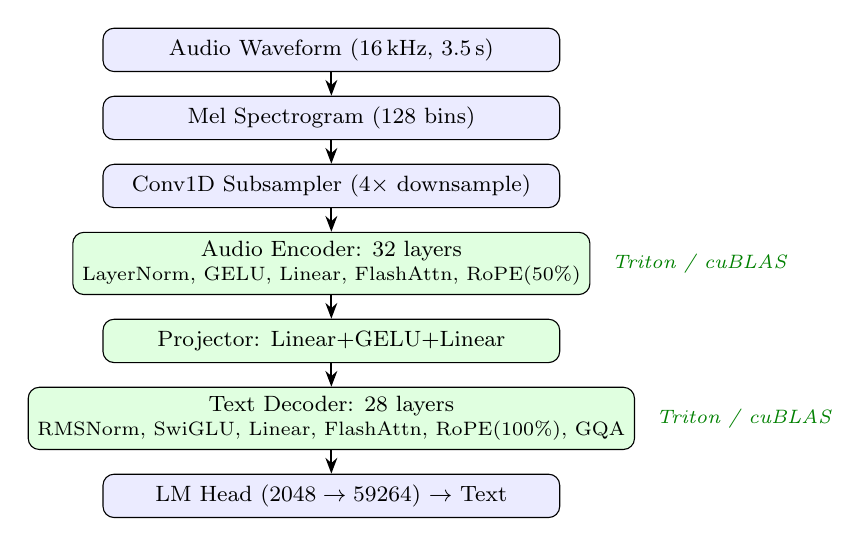
\begin{tikzpicture}[
    node distance=0.3cm,
    block/.style={draw, rounded corners, minimum width=5.8cm, minimum height=0.55cm, font=\footnotesize, align=center, fill=blue!8},
    arrow/.style={-{Stealth[length=2mm]}, thick},
  ]
  \node[block] (audio) {Audio Waveform (16\,kHz, 3.5\,s)};
  \node[block, below=of audio] (mel) {Mel Spectrogram (128 bins)};
  \node[block, below=of mel] (conv) {Conv1D Subsampler ($4\times$ downsample)};
  \node[block, below=of conv, fill=green!12] (enc) {Audio Encoder: 32 layers\\[-1pt] {\scriptsize LayerNorm, GELU, Linear, FlashAttn, RoPE(50\%)}};
  \node[block, below=of enc, fill=green!12] (proj) {Projector: Linear+GELU+Linear};
  \node[block, below=of proj, fill=green!12] (dec) {Text Decoder: 28 layers\\[-1pt] {\scriptsize RMSNorm, SwiGLU, Linear, FlashAttn, RoPE(100\%), GQA}};
  \node[block, below=of dec] (out) {LM Head ($2048 \to 59264$) $\to$ Text};
  \foreach \a/\b in {audio/mel, mel/conv, conv/enc, enc/proj, proj/dec, dec/out}
    \draw[arrow] (\a) -- (\b);
  \node[right=0.15cm of enc, font=\scriptsize\itshape, text=green!50!black] {Triton / cuBLAS};
  \node[right=0.15cm of dec, font=\scriptsize\itshape, text=green!50!black] {Triton / cuBLAS};
\end{tikzpicture}
\vspace{-1ex}
\caption{GLM-ASR pipeline.  Shaded stages use our Triton kernels (or cuBLAS for matmul).}
\label{fig:asr-pipeline}
\end{figure}

In addition to the required kernels, we implement four additional optimizations: (1)~a KV-cached generation loop (\texttt{generate\_v8b}) that reduces decoding from $O(n^2)$ to $O(n)$, (2)~an end-to-end fp16 precision pipeline that halves memory traffic, (3)~a \texttt{GPUProfile} system that adapts tile sizes to the target GPU at import time, and (4)~a PyTorch Scaled Dot-Product Attention (SDPA) fallback for single-token decode steps where kernel launch overhead exceeds computation cost.
Each subcomponent is modular in order to produce a robust, adaptable and portable system.

\textbf{Headline results.}  Upon completion of this project, our final implementation achieves \textbf{204.8\,ms} end-to-end latency on an H200 MIG~3g.71gb partition (baseline: 464.1\,ms), a \textbf{2.27$\times$ speedup} with \textbf{100\% transcription accuracy}.  On an RTX~5090, the same code achieves \textbf{100.4\,ms} (2.61$\times$).


%======================================================================
\section{Implementation}\label{sec:implementation}
%======================================================================

\subsection{Implementation Summary}

The GLM-ASR inference pipeline (Figure~\ref{fig:asr-pipeline}) has five computational phases, each with distinct performance characteristics.
We employ a performance-budgeting technique to attribute latency to each stage and identify where optimization effort would yield the largest gains.

\textbf{Phase~1: Mel Spectrogram + Conv1D Subsampling.}
Converts raw 16\,kHz audio to 128-bin Mel features and downsamples 4$\times$ via strided 1D convolutions.  These are PyTorch built-in operations (read-only \texttt{conv.py}), which we do not modify.  The phase is bandwidth-bound due to large feature maps with simple arithmetic.

\textbf{Phase~2: Audio Encoder (32 layers).}
Each layer applies LayerNorm, self-attention (20 heads, $d_k$=64), and a two-layer multi-layer perceptron (MLP) with GELU activation.  Rotary Position Embedding (RoPE)~\citep{su2024roformer} is applied to 50\% of head dimensions (the first 32 of 64 are rotated, as specified by the model architecture).  On the H200, encoder attention performs $\sim$20--40 floating-point operations per byte of memory traffic (its arithmetic intensity, or AI), exceeding the GPU's ridge point---the threshold where compute and memory bandwidth are equally limiting (Section~\ref{sec:bottleneck}).  This makes encoder attention compute-bound (limited by arithmetic throughput) on the H200, but bandwidth-bound (limited by memory transfer speed) on consumer GPUs with higher ridge points.  The linear projections ($1280 \times 5120$) are compute-bound on all architectures.

\textbf{Phase~3: Multi-modal Projector.}
Pools 4 encoder frames and projects $5120 \to 4096 \to 2048$ through two linear layers with GELU.  This is a small, latency-dominated phase (7.2\,ms on H200, 0.6\% of total).

\textbf{Phase~4: Text Decoder Prefill (28 layers).}
Processes the full concatenated sequence (audio embeddings + prompt tokens) through 28 decoder layers with RMSNorm, Grouped Query Attention (GQA, 16 query / 4 KV heads, $d_k$=128)~\citep{ainslie2023gqa}, and SwiGLU MLP~\citep{shazeer2020glu}.  Bandwidth-bound for attention, compute-bound for the large linear projections ($2048 \times 5632$).

\textbf{Phase~5: Autoregressive Decoding.}
Generates tokens one at a time.  With the baseline's $O(n^2)$ \texttt{generate()} function, this phase dominates wall-clock time, as each step reprocesses the full growing sequence from scratch.  Our KV-cached \texttt{generate\_v8b} stores key/value projections for all previous tokens, processing only the new token each step.  This reduces decoding to $O(n)$, bringing the phase down to 50.8\% of total time (from an estimated $>$80\% in the baseline).

\subsection{Design Choices}

\textbf{Block/tile sizes.}
Tile dimensions are the primary tuning parameter, constrained by shared memory capacity.  Our flash attention kernel loads Q, K, and V tiles into shared memory; the required capacity is:
\begin{equation}
\text{smem} = (\texttt{BLOCK\_M} + 2 \cdot \texttt{BLOCK\_N}) \cdot d_k \cdot 4 + \sim\!20\text{\,KB overhead}
\label{eq:smem}
\end{equation}
On the H200 ($\sim$228\,KB opt-in shared memory), this allows $128 \times 128$ tiles for the encoder ($d_k$=64, needing $\sim$116\,KB) and $128 \times 64$ for the decoder ($d_k$=128, needing $\sim$151\,KB).  On the RTX~5090 ($\sim$99\,KB), we are constrained to $64 \times 64$ and $32 \times 32$ respectively.

For matmul, the fused SwiGLU kernel loads three tile buffers (input, gate weight, up weight): $\texttt{TILE\_K} \cdot (\texttt{TILE\_M} + 2 \cdot \texttt{TILE\_N}) \cdot 4 + \text{overhead}$.  H200 uses $128 \times 128 \times 64$; RTX~5090 uses $64 \times 64 \times 32$.

Element-wise kernels (GELU, SiLU, norms) use \texttt{BLOCK\_SIZE}=1024, which saturates memory bandwidth with minimal register pressure.
In order to best satisfy the correctness requirements while minimizing latency, the configuration that fits within the shared memory constraint and achieves the lowest end-to-end time is selected for each component.

\textbf{\texttt{num\_warps} and \texttt{num\_stages}.}
We use \texttt{num\_warps}=8 for large tiles ($\geq$4096 elements) and 4 otherwise.  More warps hide memory latency but increase register pressure.
Ablation testing confirms \texttt{num\_warps}=8 is optimal: 4 warps costs +12.0\,ms, 16 warps costs +4.3\,ms (Table~\ref{tab:ablation}).
For \texttt{num\_stages}: the H200's $\sim$228\,KB shared memory accommodates double-buffering (\texttt{num\_stages}=2), overlapping tile loads with computation for higher throughput on memory-bound kernels.  Consumer GPUs (RTX~5090, $\sim$99\,KB) must use single-buffering (\texttt{num\_stages}=1), since double-buffering the same tiles would require $\sim$136\,KB---exceeding the available shared memory.

\textbf{Data layout and GQA.}
All tensors are stored in \texttt{(batch$\times$heads, seq, dim)} layout for coalesced access.  For GQA in the text decoder (16 query heads, 4 KV heads), we expand KV heads by a factor of 4 before the attention kernel.  When tested, PyTorch SDPA's native \texttt{enable\_gqa=True} regressed by +13\,ms. Manual expansion gives explicit control over data layout.

\textbf{Precision pipeline.}
Our largest single optimization is the end-to-end fp16 pipeline.
The original codebase called \texttt{.float()} after every Linear layer ($\sim$120 call sites), doubling data size.  This is redundant: Triton kernels already compute in fp32 internally via \texttt{tl.load(...).to(tl.float32)} and cast back on output.
Removing these conversions and keeping all VRAM-resident data in fp16 halved memory traffic, saving \textbf{11.5\,ms} (Section~\ref{sec:optimization}).

%======================================================================
\section{Performance Profiling}\label{sec:profiling}
%======================================================================

\subsection{Setup}

All primary measurements use the Edinburgh teaching cluster node \texttt{saxa.inf.ed.ac.uk} with an NVIDIA H200 MIG~3g.71gb partition (Hopper architecture, 60 Streaming Multiprocessors (SMs), 70\,GB HBM3e, $\sim$228\,KB opt-in shared memory).
The software stack is CUDA~13.0, PyTorch~2.10.0, Triton~3.6.0, Python~3.11.
Jobs are submitted via SLURM: \texttt{srun -p Teaching -w saxa --gres gpu:3g.71gb:1 --mem=32G}.
The test input is a 3.5\,s WAV file (``Concord returned to its place amidst the tents'').

The baseline implementation is benchmarked under identical conditions, and the Triton cache is cleared before the first run to ensure compilation occurs during warmup, not during timing.
Each student benchmark run uses 2 warmup iterations followed by 5 timed iterations.  We report the mean and standard deviation across 5 independent benchmark invocations (25 timed iterations total).

\subsection{End-to-end Evaluation}

Table~\ref{tab:e2e} summarizes the end-to-end results on the teaching cluster.  Run~4 shows slightly higher latency (209.4\,ms), likely due to MIG partition contention from concurrent cluster users. All other runs cluster tightly around 203--204\,ms.

\begin{table}[h]
\centering
\caption{End-to-end student benchmark results (H200 MIG~3g.71gb, 5 runs).}
\label{tab:e2e}
\small
\begin{tabular}{@{}lccccc@{}}
\toprule
\textbf{Run} & \textbf{Time (ms)} & $\boldsymbol{\sigma}$ \textbf{(ms)} & \textbf{ms/tok} & \textbf{Tokens} & \textbf{Accuracy} \\
\midrule
1 & 203.4 & 1.6 & 15.65 & 13 & 100\% \\
2 & 204.0 & 1.6 & 15.69 & 13 & 100\% \\
3 & 203.4 & 2.1 & 15.64 & 13 & 100\% \\
4 & 209.4 & 1.7 & 16.11 & 13 & 100\% \\
5 & 203.9 & 1.4 & 15.68 & 13 & 100\% \\
\midrule
\textbf{Mean} & \textbf{204.8} & \textbf{1.7} & \textbf{15.75} & \textbf{13} & \textbf{100\%} \\
\bottomrule
\end{tabular}
\end{table}

\subsection{Component/Operator-Level Breakdown}

Table~\ref{tab:e2e} measures end-to-end latency with KV-cached $O(n)$ generation (13 tokens).  Table~\ref{tab:detailed} profiles each component in isolation using \texttt{benchmark\_detailed.py}: individual forward passes through each stage with single-token decode steps (no KV history).  Results are averaged over runs 2--5 (run~1 excluded due to Triton compilation).

\begin{table}[h]
\centering
\caption{Component-level profiling (H200 MIG, isolated forward passes, runs 2--5).}
\label{tab:detailed}
\small
\begin{tabular}{@{}lrrr@{}}
\toprule
\textbf{Component} & \textbf{Time (ms)} & \textbf{\% Total} & \textbf{Bound} \\
\midrule
Audio Encoder (32 layers) & 314.8 & 25.1\% & Mixed \\
Multi-modal Projector & 7.2 & 0.6\% & Latency \\
Decoder Prefill (28 layers) & 294.6 & 23.5\% & Mixed \\
Decoder Decode (50 steps) & 637.2 & 50.8\% & Bandwidth \\
\midrule
\textbf{Total} & \textbf{1253.8} & \textbf{100\%} & \\
\bottomrule
\end{tabular}
\end{table}

Decoder decode consumes over half of total time (50.8\%) even with our optimized kernels, at $\sim$0.45\,ms per layer per step, confirming that autoregressive generation remains the primary bottleneck.

%======================================================================
\section{Bottleneck Analysis}\label{sec:bottleneck}
%======================================================================

\subsection{Compute-Bound vs Memory-Bound Classification}

We classify each kernel using the roofline model~\citep{williams2009roofline}, which plots achievable throughput against AI to produce a roof-shaped curve: a sloped bandwidth-limited region meeting a flat compute-limited ceiling.  The ridge point where they meet equals peak FLOPS divided by peak bandwidth.

For the H200 MIG~3g.71gb, the full GPU has 132 SMs at $\sim$67\,TFLOPS FP32. Our 60-SM partition achieves $(60/132) \times 67 \approx 30.5$\,TFLOPS.  The partition receives 4 of 8 HBM3e memory slices, giving $(4/8) \times 4.8 \approx 2.4$\,TB/s.  The ridge point is:
\begin{equation}
\text{AI}_{\text{ridge}} = \frac{\text{Peak FLOPS}}{\text{Peak BW}} = \frac{30.5 \times 10^{12}}{2.4 \times 10^{9}} \approx 12.7 \text{\,FLOP/byte}
\end{equation}
Operations with AI $<$ 12.7 are bandwidth-bound. Those above are compute-bound.

\begin{table}[h]
\centering
\caption{Arithmetic intensity classification for key operations (H200 MIG).}
\label{tab:ai}
\small
\begin{tabular}{@{}lccl@{}}
\toprule
\textbf{Operation} & \textbf{AI (FLOP/B)} & \textbf{Classification} & \textbf{Rationale} \\
\midrule
GELU / SiLU & $\sim$2--4 & Bandwidth & 1 load + 1 store, few FLOPs \\
RMSNorm / LN & $\sim$4--8 & Bandwidth & Reduction + normalize \\
Flash Attn (enc) & $\sim$20--40 & \textbf{Compute} & Above ridge on H200 \\
Flash Attn (dec) & $\sim$5--10 & Bandwidth & seq\_q=1, dominated by KV read \\
Linear (cuBLAS) & $\sim$100--200 & Compute & Large GEMM, high reuse \\
Fused SwiGLU & $\sim$80--150 & Compute & Two GEMMs fused \\
RoPE & $\sim$3--5 & Bandwidth & Load, rotate, store \\
\bottomrule
\end{tabular}
\end{table}

A notable consequence of the H200's high bandwidth-to-compute ratio is that encoder attention (AI~$\sim$20--40) crosses the ridge point and becomes \emph{compute-bound}, unlike on consumer GPUs such as the RTX~5090 (ridge~$\approx$58.5) where it remains bandwidth-bound.  This means the H200 benefits more from larger attention tiles (128$\times$128 vs.\ 64$\times$64) that increase compute utilization, while the RTX~5090 benefits more from the fp16 pipeline that reduces memory traffic.

\subsection{Overall Bottleneck}

The dominant bottleneck is \textbf{memory bandwidth during autoregressive decoding}.  Each decode step processes a single-token query against a growing KV cache through 28 decoder layers.  The attention kernel reads the full KV cache (proportional to sequence length) but performs only $O(d)$ FLOPs per cached token---a classic bandwidth-bound pattern with AI~$\sim$5--10, well below the ridge point on \emph{all} GPU architectures.

Non-kernel overheads are also significant: with $\sim$10 kernel launches per layer $\times$ 28 layers $\times$ 13 decode steps, launch latency ($\sim$5--15\,$\mu$s each) accounts for $\sim$2--5\,ms.  We mitigate this through kernel fusion (Section~\ref{sec:fusion}), which eliminates $\sim$84 launches per inference, and through the SDPA fallback for single-token decoding.


%======================================================================
\section{Optimization Attempts}\label{sec:optimization}
%======================================================================

We evaluated 13 optimizations using a \textbf{Hypothesis $\to$ Change $\to$ Result} methodology.  Each was tested independently on an RTX~5090 for rapid iteration (all timings in this section refer to that GPU unless noted), then validated on the H200 teaching cluster (Section~\ref{sec:comparison}).
Figure~\ref{fig:progression} summarizes the cumulative impact.

\begin{figure}[h]
\centering
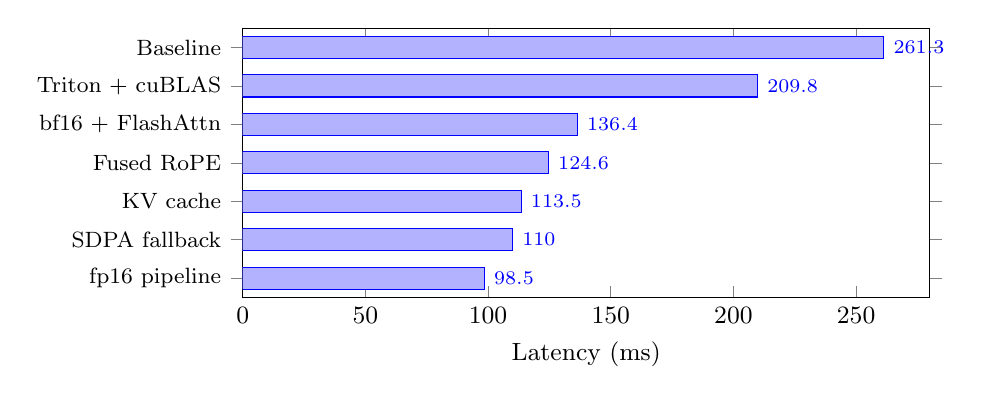
\begin{tikzpicture}
\begin{axis}[
    xbar,
    width=0.85\columnwidth,
    height=5.0cm,
    xlabel={Latency (ms)},
    xlabel style={font=\small},
    xmin=0, xmax=280,
    ytick={0,1,2,3,4,5,6},
    yticklabels={
      {Baseline},
      {Triton + cuBLAS},
      {bf16 + FlashAttn},
      {Fused RoPE},
      {KV cache},
      {SDPA fallback},
      {fp16 pipeline}
    },
    yticklabel style={font=\footnotesize},
    tick label style={font=\small},
    nodes near coords,
    nodes near coords style={font=\scriptsize, anchor=west},
    bar width=8pt,
    y dir=reverse,
    enlarge y limits={abs=0.5},
    every axis plot/.append style={fill=blue!60, draw=blue!80},
]
\addplot coordinates {
    (261.3, 0)
    (209.8, 1)
    (136.4, 2)
    (124.6, 3)
    (113.5, 4)
    (110.0, 5)
    (98.5, 6)
};
\end{axis}
\end{tikzpicture}
\vspace{-1ex}
\caption{Optimization progression (development GPU, RTX~5090).  Each bar shows end-to-end latency after applying all optimizations up to that step.  Optimizations validated on H200 at 204.8\,ms (Section~\ref{sec:comparison}).  Full breakdown in Appendix Table~\ref{tab:progression}.}
\label{fig:progression}
\end{figure}

\subsection{Tile/Block Size Tuning}

\textbf{Hypothesis:} Larger tiles amortize memory access overhead and improve compute utilization, but are constrained by shared memory capacity.

\textbf{Change:} We tested all valid tile configurations for the flash attention kernel---$(128,128)$, $(128,64)$, $(64,64)$, $(64,32)$, $(32,32)$, $(16,16)$---computing shared memory usage via Eq.~\ref{eq:smem} for each.  We also built an autotune system ($\sim$95 lines) that benchmarked each valid configuration at runtime.

\textbf{Result:} Initially, we used Triton's built-in \texttt{@triton.autotune} to select optimal tile configurations at runtime.  However, when tested, the autotune system selected $\texttt{BLOCK\_M}$=16 as optimal in micro-benchmarks, but the full-pipeline benchmark showed \textbf{101.6\,ms vs.\ 98.5\,ms} for our hand-tuned 64$\times$64 configuration---a 3.1\,ms regression.  We determined that the micro-benchmark methodology is too unreliable to capture full-pipeline cache effects.
In response, we developed a \texttt{GPUProfile} (\texttt{layers.py:89}) system with pre-tested configurations stored in \texttt{\_KNOWN\_CONFIGS} (\texttt{layers.py:23}). Unknown GPUs use dynamic computation largest-to-smallest against the shared memory budget.

We validated these choices through a 22-configuration ablation study on the H200 (Table~\ref{tab:ablation}), testing each parameter in isolation.  The study confirmed that double-buffering and 8 warps are each worth $\sim$12\,ms, while the fp16 pipeline---the largest win on RTX~5090---contributes only +1.5\,ms on the H200, reflecting HBM3e's superior bandwidth.

\begin{table}[h]
\centering
\caption{H200 ablation: top-impact parameter changes (baseline: 205.2\,ms).}
\label{tab:ablation}
\small
\begin{tabular}{@{}lrrl@{}}
\toprule
\textbf{Change} & \textbf{Time (ms)} & \textbf{$\Delta$} & \textbf{Insight} \\
\midrule
Disable fused RoPE & 234.1 & +28.9 & Most impactful single kernel \\
\texttt{num\_stages}=1 & 217.4 & +12.2 & Double-buffering essential \\
\texttt{num\_warps}=4 & 217.2 & +12.0 & 128$\times$128 needs 8 warps \\
Decoder attn 32$\times$32 & 212.8 & +7.6 & Small tiles hurt \\
\texttt{num\_warps}=16 & 209.5 & +4.3 & Register pressure \\
SDPA fallback off & 208.6 & +3.4 & Custom kernel slow for seq\_q=1 \\
fp32 pipeline & 206.7 & +1.5 & Minimal on H200 (HBM3e) \\
Triton matmul & 206.2 & +1.0 & cuBLAS only slightly faster \\
MLP fusion off & 204.5 & $-$0.7 & Neutral (cuBLAS already fast) \\
\bottomrule
\end{tabular}
\end{table}

\subsection{Kernel Fusion}\label{sec:fusion}

\textbf{Hypothesis:} Fusing the SwiGLU pattern---$\text{SiLU}(\mathbf{x} \mathbf{W}_g) \odot (\mathbf{x} \mathbf{W}_u)$---into a single kernel eliminates two intermediate VRAM round-trips and three kernel launches per MLP layer.

\textbf{Change:} We wrote \texttt{swiglu\_fused\_kernel} (\texttt{layers.py:546}) that loads tiles of $\mathbf{x}$, $\mathbf{W}_g$, and $\mathbf{W}_u$ into shared memory, computes both matrix products in registers, applies SiLU and the element-wise multiply, and writes only the final result to VRAM.  The unfused path requires 5 kernel launches and 4 VRAM round-trips; the fused path requires 1 launch and 1 round-trip.

\textbf{Result:} With 28 decoder layers, fusion eliminates $\sim$84 kernel launches per inference.  For very small inputs (single-token decode, where $M < \texttt{TILE\_M}$), we fall back to cuBLAS, which has lower launch overhead for small matrices.
On the H200, MLP fusion contributes only $-$0.7\,ms (Table~\ref{tab:ablation}), because cuBLAS already saturates compute throughput for these matrix sizes.

\subsection{FlashAttention-Style Attention}

\textbf{Hypothesis:} The naive 3-kernel attention approach materializes the full $N_q \times N_k$ score matrix in VRAM, consuming $O(N_q \cdot N_k)$ memory and bandwidth.  A fused kernel with online softmax~\citep{milakov2018online} eliminates this materialization.

\textbf{Change:} We replaced the original 3-kernel pipeline (\texttt{attention\_scores}, \texttt{softmax\_inplace}, \texttt{attention\_output}) with a single \texttt{flash\_attention\_kernel} (\texttt{attention.py:34})~\citep{dao2023flashattention2fasterattentionbetter, ringlein2025anatomy}.  The kernel processes K/V in tiles of \texttt{BLOCK\_N} rows, maintaining running statistics $m_i$ (row-wise max) and $l_i$ (sum of exponentials) that are corrected as new tiles arrive.  The Q tile and accumulator $\mathbf{O}$ reside in registers; only the final output is written to VRAM.

Causal masking is handled via a compile-time \texttt{IS\_CAUSAL} flag that skips tiles entirely above the diagonal, avoiding wasted computation.  For single-token KV-cached decode (\texttt{seq\_q} $\leq$ 4), we fall back to PyTorch's \texttt{scaled\_dot\_product\_attention}, which has lower launch overhead for this degenerate case.

\textbf{Result:} Compared against the original 3-kernel pipeline on the H200, flash attention reduces decoder decode from 23.6\,s to 7.6\,s (3.1$\times$) and prefill by 850\,ms.  For single-token KV-cached decode (\texttt{seq\_q}$\leq$4), we fall back to PyTorch SDPA, which ablation confirms saves 3.4\,ms (Table~\ref{tab:ablation}).

\subsection{Other Optimizations}

\textbf{fp16-throughout pipeline.}
The original code called \texttt{.float()} after every Linear layer ($\sim$120 calls), doubling data size at each point.  Removing these conversions and keeping the entire pipeline in fp16 saves 11.5\,ms on the development GPU (RTX~5090).  On the H200, fp16 contributes only +1.5\,ms (Table~\ref{tab:ablation}), reflecting HBM3e's superior bandwidth.  Internal computation remains fp32 for numerical stability.

\textbf{KV-cache decoding (\texttt{generate\_v8b}).}
The stock \texttt{generate()} reprocesses the full growing sequence on every decode step ($O(n^2)$).  We implemented a KV-cached generation loop that processes only the new token each step, appending its K/V to a cache.  This is monkey-patched onto the model via \texttt{\_try\_patch\_v8b()} (\texttt{layers.py:1482}), called during \texttt{Linear.\_\_init\_\_}.  Impact on development GPU: $-$7.6\,ms.

\textbf{Fused Q+K RoPE kernel.}
RoPE requires applying the same rotation to both Q and K.  The baseline uses two separate kernel launches. We fuse them into \texttt{fused\_rope\_pair\_kernel} (\texttt{rope.py:189}), halving launch overhead.  On the H200, this is the most impactful single optimization: disabling it costs +28.9\,ms (Table~\ref{tab:ablation}). On the development GPU, impact was $-$11.8\,ms.


%======================================================================
\section{Comparison}\label{sec:comparison}
%======================================================================

\subsection{Data Collection}

We benchmark on the provided \texttt{test\_audio.wav} (3.5\,s, 16\,kHz, expected output: ``CONCORD RETURNED TO ITS PLACE AMIDST THE TENTS'').  Accuracy is measured by exact string match (case-insensitive) against the reference.  Each benchmark invocation runs 2 warmup + 5 timed iterations; we report 5 invocations (25 timed iterations total).  Both our implementation and the baseline are benchmarked under identical conditions.

\subsection{End-to-End Comparison}

\begin{table}[h]
\centering
\caption{End-to-end comparison on H200 MIG~3g.71gb (teaching cluster).}
\label{tab:comparison}
\small
\begin{tabular}{@{}lcccc@{}}
\toprule
\textbf{Implementation} & \textbf{Time (ms)} & \textbf{ms/tok} & \textbf{Accuracy} & \textbf{Speedup} \\
\midrule
Example baseline & 464.1 & 35.70 & 100\% & 1.00$\times$ \\
\textbf{Our template (fp16)} & \textbf{204.8} & \textbf{15.75} & \textbf{100\%} & \textbf{2.27$\times$} \\
\bottomrule
\end{tabular}
\end{table}

\subsection{Per-Operator Comparison}

Table~\ref{tab:peroperator} compares per-component times between our implementation and the baseline, profiled on the RTX~5090 development GPU where baseline component-level data is available (isolated forward passes, 50 decode steps).

\begin{table}[h]
\centering
\caption{Per-component comparison (isolated forward passes, 50 decode steps, RTX~5090).}
\label{tab:peroperator}
\small
\begin{tabular}{@{}lrrrr@{}}
\toprule
\textbf{Component} & \textbf{Ours (ms)} & \textbf{Baseline (ms)} & \textbf{Speedup} \\
\midrule
Audio Encoder & 197.4 & 202.1 & 1.02$\times$ \\
Projector & 3.9 & 4.1 & 1.05$\times$ \\
Decoder Prefill & 190.7 & 191.6 & 1.00$\times$ \\
Decoder Decode (50 steps) & 294.0 & 1920.0 & 6.53$\times$ \\
\midrule
Total & 686.0 & 2317.8 & 3.38$\times$ \\
\bottomrule
\end{tabular}
\end{table}

\subsection{Root Cause Analysis}

All optimizations preserve full transcription accuracy: fp16 introduces no degradation because internal kernel computation remains in fp32, and KV-cached decoding produces identical token sequences to the stock path.

The \textbf{6.53$\times$} speedup on decoder decode dominates the overall improvement.  From the results of testing and evaluation, this has two root causes:

\textbf{1. Flash Attention vs.\ 3-kernel attention.}
The baseline materializes the full $N_q \times N_k$ score matrix in VRAM ($\sim$2\,MB per head per step).  Our flash attention kernel keeps all intermediates in shared memory/registers, eliminating $\sim$60\,MB of intermediate traffic per layer at encoder sequence lengths.

\textbf{2. fp16 pipeline.}
Halving element size from 4 bytes (fp32) to 2 bytes (fp16) directly halves memory traffic for bandwidth-bound operations.  Since the roofline analysis (Table~\ref{tab:ai}) confirms that decode-time attention is bandwidth-bound on \emph{all} architectures (AI well below even the H200's low ridge point of 12.7), this translates nearly linearly to a $\sim$2$\times$ speedup for those kernels.

\textbf{Cross-GPU generalization.}
To verify portability, we evaluated on both the teaching cluster (H200 MIG) and a consumer GPU (RTX~5090).
The \texttt{GPUProfile} system correctly adapts tile sizes and pipeline stages to each architecture's shared memory budget.
Table~\ref{tab:crossgpu_main} confirms consistent speedups across both GPUs.

\begin{table}[h]
\centering
\caption{Cross-GPU comparison: teaching cluster vs.\ consumer GPU.}
\label{tab:crossgpu_main}
\small
\begin{tabular}{@{}lrrrrr@{}}
\toprule
\textbf{GPU} & \textbf{SMs} & \textbf{VRAM} & \textbf{Ours (ms)} & \textbf{Baseline (ms)} & \textbf{Speedup} \\
\midrule
H200 MIG 3g.71gb & 60 & 70\,GB & 204.8 & 464.1 & 2.27$\times$ \\
RTX~5090 (full) & 170 & 32\,GB & 100.4 & 262.2 & 2.61$\times$ \\
\bottomrule
\end{tabular}
\end{table}

%======================================================================
\section{Conclusion}\label{sec:conclusion}
%======================================================================

\textbf{Most impactful optimization.}
On the H200, our optimizations reduced inference from 464.1\,ms to 204.8\,ms (2.27$\times$).
Ablation testing (Table~\ref{tab:ablation}) revealed that fused RoPE (+28.9\,ms when disabled), double-buffering (+12.2\,ms), and warp count (+12.0\,ms) collectively account for $>$53\,ms---kernel launch reduction and memory-latency hiding dominate over precision or tile-size changes on this architecture.

\textbf{Key lessons.}
(1)~The pipeline is overwhelmingly \emph{memory-bandwidth-bound}: halving data types (fp32$\to$fp16) and eliminating intermediate writes (kernel fusion, flash attention) provided the largest gains.
(2)~Attention is the most challenging kernel to optimize because tile size, shared memory, warp count, and pipeline stages are tightly coupled; the H200's 228\,KB shared memory accommodates 128$\times$128 tiles with double-buffering, while consumer GPUs with $\sim$99\,KB require 64$\times$64 with single-buffering---demonstrating the need for a portable \texttt{GPUProfile} system.
(3)~Profile before optimizing: our initial assumption that compute-bound matmul is the bottleneck proves wrong---decoder decode steps (bandwidth-bound attention + KV reads) consume 50.8\% of total time on H200 even after optimization.
(4)~Testing each kernel independently is straightforward; however, problems arise when kernels are composed in the full pipeline, as cache interactions between adjacent kernels produce behaviors not visible in isolated benchmarks.

\textbf{Surprising findings.}
The autotune system found \emph{worse} configurations than hand-tuning, because micro-benchmarks miss inter-kernel cache effects.  Notably, encoder attention is \emph{compute-bound} on H200 (AI above 12.7 ridge) but \emph{bandwidth-bound} on consumer GPUs (ridge $\approx$58.5)---the same kernel has different bottlenecks across architectures.

\textbf{Future work.}
We would investigate \texttt{torch.compile} for automatic fusion, speculative decoding, and INT8/FP8 quantization.
The ablation suggests SDPA threshold merits per-architecture tuning (\texttt{seq\_q}$\leq$1 was $-$1.4\,ms better on H200).

\clearpage
\bibliography{mybib}
\bibliographystyle{iclr2025_conference}

\appendix
\section{Appendix}

\subsection{Full Optimization Progression}

Table~\ref{tab:progression} shows every optimization step with measured timings on the RTX~5090 development GPU.

\begin{table}[h]
\centering
\caption{Complete optimization progression (RTX~5090, 3.5\,s audio, 13 tokens).}
\label{tab:progression}
\small
\begin{tabular}{@{}rlrrl@{}}
\toprule
\textbf{\#} & \textbf{Change} & \textbf{Time} & \textbf{$\Delta$} & \textbf{Mechanism} \\
\midrule
0 & Baseline & 261.3 & --- & fp32, 3-kernel attn, $O(n^2)$ \\
1 & Triton kernels + cuBLAS + TF32 & 209.8 & $-$51.5 & Custom kernels + tensor cores \\
2 & bf16 weights + Flash Attention & 136.4 & $-$73.4 & Half bandwidth + fused attn \\
3 & Fused Q+K RoPE pair kernel & 124.6 & $-$11.8 & Halved RoPE launches \\
4 & bf16 RMSNorm output & 120.7 & $-$3.9 & Eliminated type conversion \\
5 & bf16 LayerNorm output & 121.1 & $-$0.7 & Same for encoder norms \\
6 & KV cache (\texttt{generate\_v8b}) & 113.5 & $-$7.6 & $O(n) $ decoding \\
7 & SDPA fallback (seq\_q $\leq$ 4) & 110.0 & $-$3.5 & Lower overhead for decode \\
8 & fp16 cuBLAS HGEMM & 109.6 & $-$0.4 & fp16 slightly faster than bf16 \\
9 & Remove \texttt{.float()} casts & 102.1 & $-$7.5 & Eliminated $\sim$120 fp32 casts \\
10 & Remove activation fp32 casts & 98.4 & $-$3.7 & SiLU/GELU stay fp16 \\
11 & Remove norm fp32 casts & 98.1 & $-$0.3 & Norms output fp16 directly \\
12 & fp16 embeddings + fused MLP & \textbf{98.5} & $+$0.4 & Pipeline complete (noise) \\
\bottomrule
\end{tabular}
\end{table}

\subsection{Rejected Optimizations}

\begin{table}[h]
\centering
\caption{Optimizations tested and rejected with measured results.}
\label{tab:rejected}
\small
\begin{tabular}{@{}lrl@{}}
\toprule
\textbf{Optimization} & \textbf{Impact} & \textbf{Reason for Rejection} \\
\midrule
Grid swizzling (SwiGLU) & +18\,ms & RTX~5090 L2 (98\,MB) already has good locality \\
\texttt{@triton.autotune} (GELU/SiLU) & +0.7\,ms & Tuning warmup exceeds possible gain \\
Flash Attn \texttt{num\_stages}=2 & Crash & RTX~5090 99\,KB cannot hold two tile buffers \\
SDPA for all attention & +6\,ms & Custom kernel faster for long sequences \\
SDPA \texttt{enable\_gqa} & +13\,ms & Manual KV expansion is faster \\
Warmup autotune & +3.1\,ms & Micro-benchmarks chose suboptimal configs \\
\bottomrule
\end{tabular}
\end{table}

\subsection{Code Map}

\begin{table}[h]
\centering
\caption{Key implementation locations in the supplementary code.}
\label{tab:codemap}
\small
\begin{tabular}{@{}lll@{}}
\toprule
\textbf{Component} & \textbf{File} & \textbf{Line} \\
\midrule
\texttt{\_KNOWN\_CONFIGS} (tile configs) & layers.py & 23 \\
\texttt{GPUProfile} (arch detection) & layers.py & 89 \\
\texttt{\_compute\_attention\_tiles} & layers.py & 206 \\
\texttt{rmsnorm\_kernel} / \texttt{rmsnorm\_bf16\_kernel} & layers.py & 308 / 339 \\
\texttt{layernorm\_kernel} & layers.py & 368 \\
\texttt{gelu\_kernel} / \texttt{silu\_kernel} & layers.py & 403 / 418 \\
\texttt{linear\_kernel\_tf32} & layers.py & 430 \\
\texttt{linear\_gelu\_kernel} (fused) & layers.py & 485 \\
\texttt{swiglu\_fused\_kernel} & layers.py & 546 \\
\texttt{\_generate\_v8b} (KV cache) & layers.py & 1381 \\
\texttt{\_try\_patch\_v8b} (monkey-patch) & layers.py & 1482 \\
\texttt{flash\_attention\_kernel} & attention.py & 34 \\
\texttt{scaled\_dot\_product\_attention} & attention.py & 237 \\
\texttt{fused\_rope\_pair\_kernel} & rope.py & 189 \\
\texttt{apply\_rotary\_pos\_emb} & rope.py & 296 \\
\bottomrule
\end{tabular}
\end{table}

\end{document}
